\chapter{Problématiques émergentes}

\section{Orientations de recherche}

In this paper we described different design principles and context models for
context-aware systems and presented various existent middleware and
server-based approaches to ease the configuration of context-aware application.

There are several research areas involved in the development of context-based
configuration. Here are three of the most relevant :

\subsection{Middleware and implementation details}

The need for new middleware arises on the implementation side. Current
middleware technologies are not adequate to handle the resctrictions imposed by
mobility and smart environmental systems : volatile connections, processing and
memory restrictions on mobile devices, narrow communication channels, reduced
screens, restricted input mechanisms, and the list goes on. There are a set of 
contex-aware imlementations in litterature with some working prototypes :

\begin{itemize}
    \item \textbf{Hydrogen} \cite{Hofer2002}: a three layer architecture
    \item \textbf{Gaia} \cite{Chetan2005}: another middleware infrastructure,
    extends typical operating system concepts to include context-awareness.
    \item \textbf{CybreMinder} \cite{Abowd2002}: a context-aware system for sup-
    porting reminders
    \item \textbf{Context Toolkit} \cite{Dey2001}: a widget based architecture
\end{itemize}

\subsection{Representation of context-information}

The representation of context-information is another concern. We presented in
this paper a generic ontology approach. It is based on four main concepts: user,
environment, platform and resources.  Presently, ontologies are mainly employed
to enable communication across the different devices in the same network. As
proposed by ContextUML \cite{Sheng2005}, the Unified Modeling Language (UML) can
also be used to model context. The models could be used to separate the
definition and information related to the context from the specific
implementation. There are other characteristics that make context information
difficult to model, as stated before, it is sometimes necessary to differentiate
between static and dynamic information.


L'une des principales innovations à apporter dans les infrastructures
d'applications sensibles au contexte réside dans l'introduction d'une interface
présentant un niveau d'abstraction élevé. Cela permetterait de représenter la
connectivité des composants applicatifs avec les politiques de haut niveau qui
la régissent.  Cette couche doit rester simple d'utilisation pour les
développeurs d'applications, et le modèle améliorer simultanément
l'automatisation et la sécurité.

\section{Ontologie de contexte}

\section{Théorie de promesse}

Le modèle permettant la définition des politiques d'administration serait un
modèle orienté sur les ontologies et basé sur la théorie de la promesse.
Celle-ci s'appuie sur un contrôle évolutif des objets intelligents,
contrairement aux modèles impératifs plus traditionnels pensés comme des
systèmes de gestion descendants.  Dans ces derniers, le gestionnaire central
doit être informé des commandes de configuration des objets sous-jacents et de
l'état actuel de ces objets.

Au sein du contexte, le modèle fournit une série d'objets qui définissent
l'application. Les objets englobent les terminaux, les groupes de terminaux et
les politiques qui définissent leur relation.

L'infrastructure conçoit un modèle d'objet pour le déploiement d'applications,
ces dernières constituant le point central. Historiquement, les applications
étaient limitées par les capacités du réseau et par des configurations visant à
prévenir leur utilisation abusive. Des concepts tels que l'adressage, le VLAN et
la sécurité sont depuis toujours intimement liés, ce qui limite l'évolutivité et
la mobilité des applications. Alors que les applications sont redessinées pour
la mobilité et l'évolutivité web, cette approche traditionnelle empêche leur
déploiement rapide et homogène.

\subsection{Principes de fonctionnement}

\section{Algorithmes de consensus}

\subsection{Algorithme de Paxos}

\subsection{Algorithme de Raft}

Raft est un algorithme de consensus qui est conçu pour être facile à comprendre.
Il est équivalent à Paxos dans la tolérance aux pannes et en termes de
performance. La différence, c'est qu'il est décomposé en sous-problèmes
relativement indépendants, et il traite de manière rigoureuse toutes les pièces
majeures nécessaires pour obtenir un système cohérent.

Le consensus est un problème fondamental dans les systèmes distribués tolérants
aux pannes. Consensus implique de multiples serveurs acceptant des valeurs. Une
fois qu'ils atteignent une décision sur une valeur, cette décision est
définitive. Les algorithmes de consensus typiques  sont amenés à faire des
progrès lorque la majorité de leurs serveurs sont disponibles, par exemple, un
cluster de 5 serveurs peut continuer à fonctionner même si deux serveurs ne sont
plus disponibles. Si plusieurs serveurs échouent, ils cessent de faire des
progrès (mais ils ne retournerons jamais de valeurs érronées)

\section{Vue d'ensemble}

Comme on le voit \ref{archi}

\begin{figure}[ht!]
  \centering
  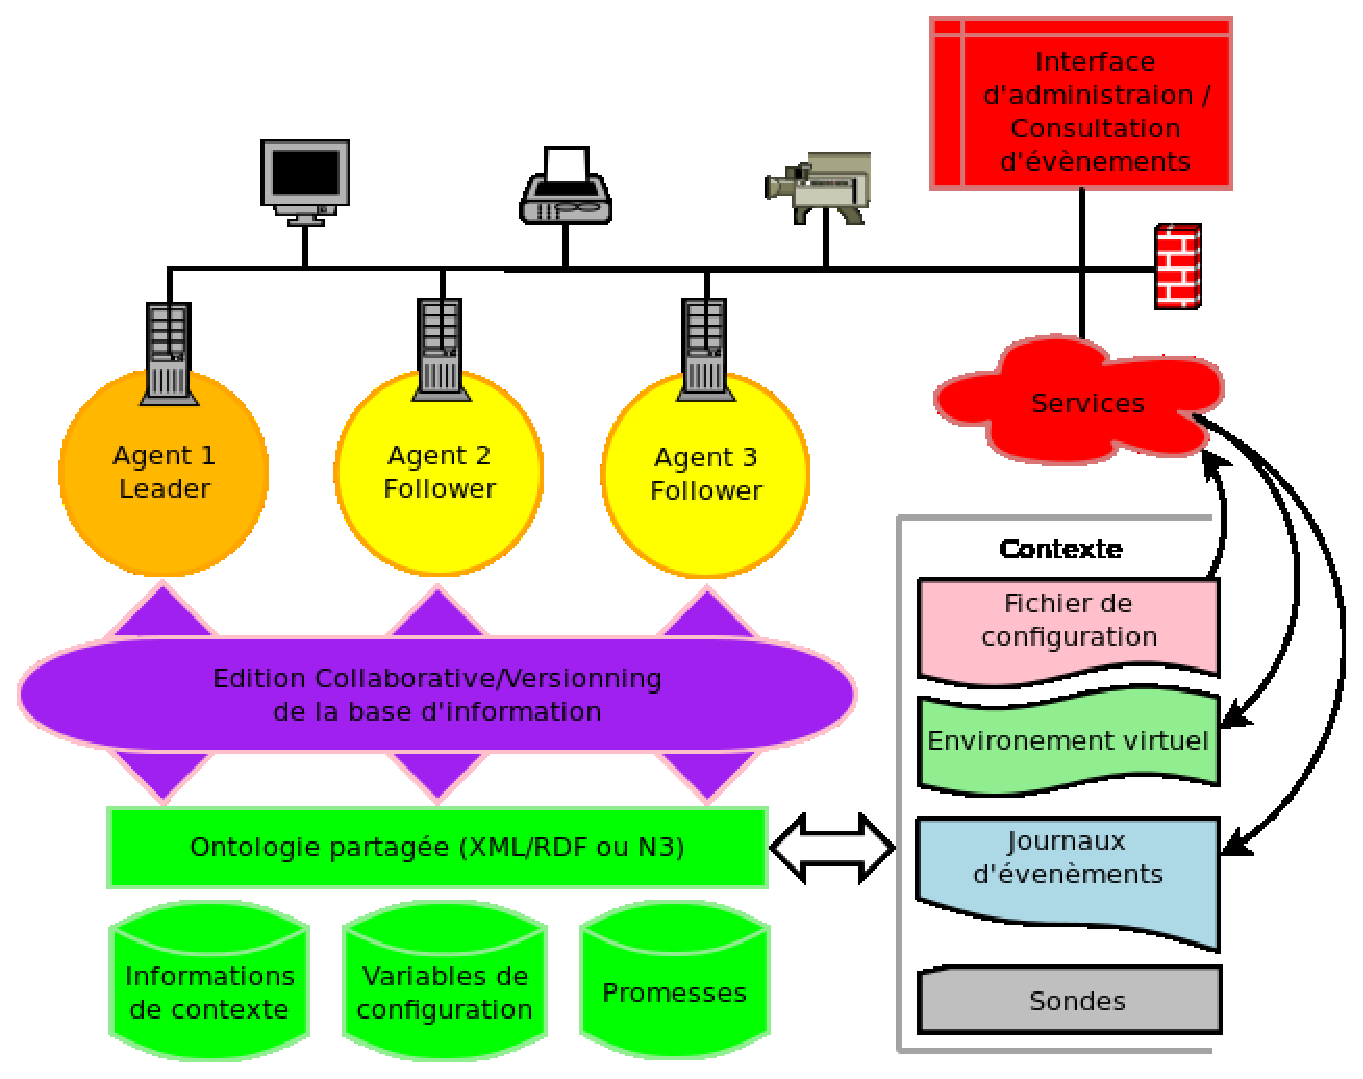
\includegraphics[width=90mm]{img/archi}
  \caption{Schéma d'implémentation du système multi-agents}
  \label{archi}
\end{figure}
